\documentclass{article}
\usepackage{times}
\usepackage[nohead,bottom=3cm,top=2cm,a4paper]{geometry}
\usepackage{xcolor}
\usepackage{graphicx}
\usepackage[nswissgerman]{babel}
\usepackage{listings}
\usepackage{blindtext}
\usepackage{lipsum}

\usepackage{amssymb}    % math symbols
\usepackage{amsmath}    % math symbols
\graphicspath{ {./results/} }


\title{Bericht aus dem Projekt sleepCube, Vorlesung: Rechenarchitektur \& vertrauenwürdiges Rechnen}
\author{von Ugur Turhal, Berkan Kurt \& Silvan Lenzlinger}
\begin{document}
\maketitle
In diesem Dokument ist der Schlussbericht. Aus Übersichtlichkeit, ist ein zusätzliches Dokument für die Programmierung erstellt, es wird in den nötigen Stellen darauf verviewiesen. In diesem ist der Quellcode für die eigenständig geschrieben Programme enthalten. 

%%%%
\section*{Sammeln der Daten}
\paragraph{Daten}
\begin{center}
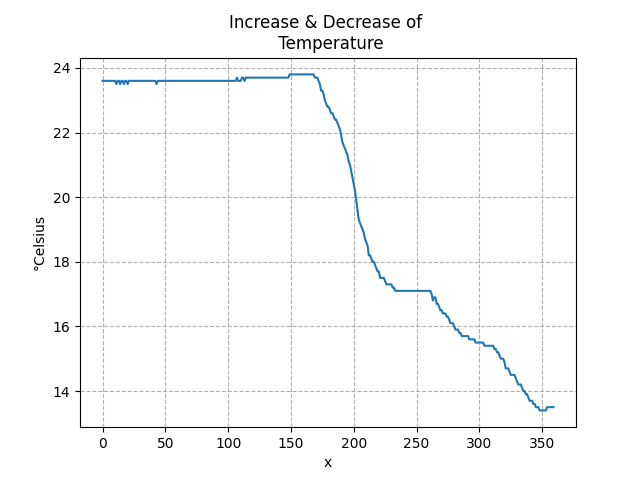
\includegraphics[width=0.49\textwidth]{plot.png}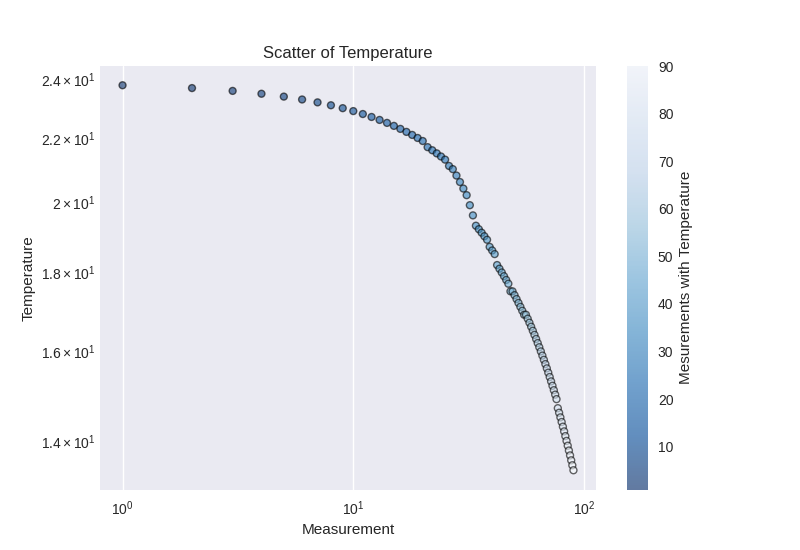
\includegraphics[width=0.53\textwidth]{scatter.png}
\end{center}

\begin{center}
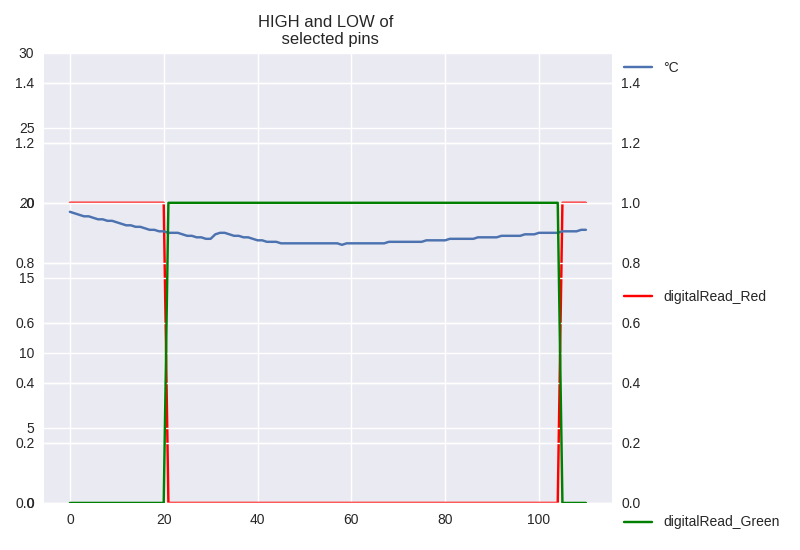
\includegraphics[width=0.53\textwidth]{digitalRead.png}
\end{center}

\paragraph{Vorteil durch die Daten}
\section*{Aufbauen des Cubes}



%%%%
\section*{Programmierung des Cubes}

%%%%
\section*{Generelle Probleme}




\end{document}
